\chapter{Distribución de probabilidad de la amplitud y fase del dipolo}

En el trabajo \cite{linsley1975fluctuation} se estudia los límites de confianza para la amplitud y la fase obtenidos mediante el análisis del primer armónico en Fourier. Las fórmulas que se describen a continuación describen a un conjunto de N mediciones cuya anisotropía está caracterizada por el vector $\vec{s}$ con una dispersión $\sigma = \sqrt{\nicefrac{2}{N}}$, sin pérdida de generalidad debido a la periodicidad de la fase, la misma puede considerarse nula. Este vector puede ser obtenido mediante distintos métodos, en este trabajo se  utilizaron el método de Rayleigh e East - West.

La distribución de probabilidad de la amplitud y la fase está dada por la Ec.\ref{eq:full_pdf}. Las variables $r$ y $\psi$ representan las variaciones de las medidiones con respecto a $\vec{s}$
\begin{equation}
    p(r,\psi) =dr\,d\psi\,\frac{r}{2\pi\sigma^2}\exp{ -\frac{(r^2+s^2 - 2rs\cos\psi)}{2\sigma^2} } \label{eq:full_pdf}
\end{equation}  

\section{Distribución de probabilidad de la amplitud}

Integrando la Ec.\ref{eq:full_pdf} con respecto a $\psi$, se obtiene la función de densidad de probabilidad $p(r)$ y el nivel de confianza $CL(s)$.
\begin{align}
    p(r) &=\frac{r}{\sigma^2}\exp{ -\frac{(r^2+s^2)}{2\sigma^2} }K_0(\frac{rs}{\sigma^2})    \label{ec:pdf}\\
    CL_r(r_0,r_1s) &= \int_{r_0}^{r_1} dr \, p(r)
    \label{ec:integral}
\end{align}  
Estas ecuaciones nos permiten determinar el nivel de confianza $CL$ con el cual se puede afirmar que el módulo del dipolo se encuentra entre los valores $r_0$ y $r_1$.

Se define el valor $r^{UL}$ como el límite superior donde se  puede afirmar que el módulo de dipolo se encuentra entre 0 y $r^{UL}$ con un $99\%$ de certeza.

\begin{align}
    CL_r(0,r^{UL},s) = 0.99 = \int_{0}^{r^{UL}} dr \, p(r)
    \label{ec:r_upper_limit}
\end{align} 
% Para alcanzar un  nivel del confianza  del  CL[\%] \footnote{ Donde CL=.99 para un 99\% o CL=0.68 para un 68\%,},  se toma el valor de amplitud $r^{UL}$ y la integral de la función \ref{ec:pdf} desde 0 hasta $r^{UL}$, donde el resultado debe ser el nivel de confianza CL.
% \begin{align}
%     CL = \int_{0}^{r^{UL}} dr \frac{r}{\sigma^2}\exp{\Big( -\frac{(r^2+s^2)}{2\sigma^2} + \frac{rs}{\sigma^2}\Big)}K_0(\frac{rs}{\sigma^2})
%     \label{ec:integral}
% \end{align}
Suponiendo que mediante el análisis de un conjunto de eventos, se obtiene que $s=0.005$ y $\sigma=0.038$. El gráfico de la función $p(r)$ y el límite de confianza en función de $r$ se muestra a continuación:

\begin{figure}[H]
    \begin{small}
        \begin{center}
            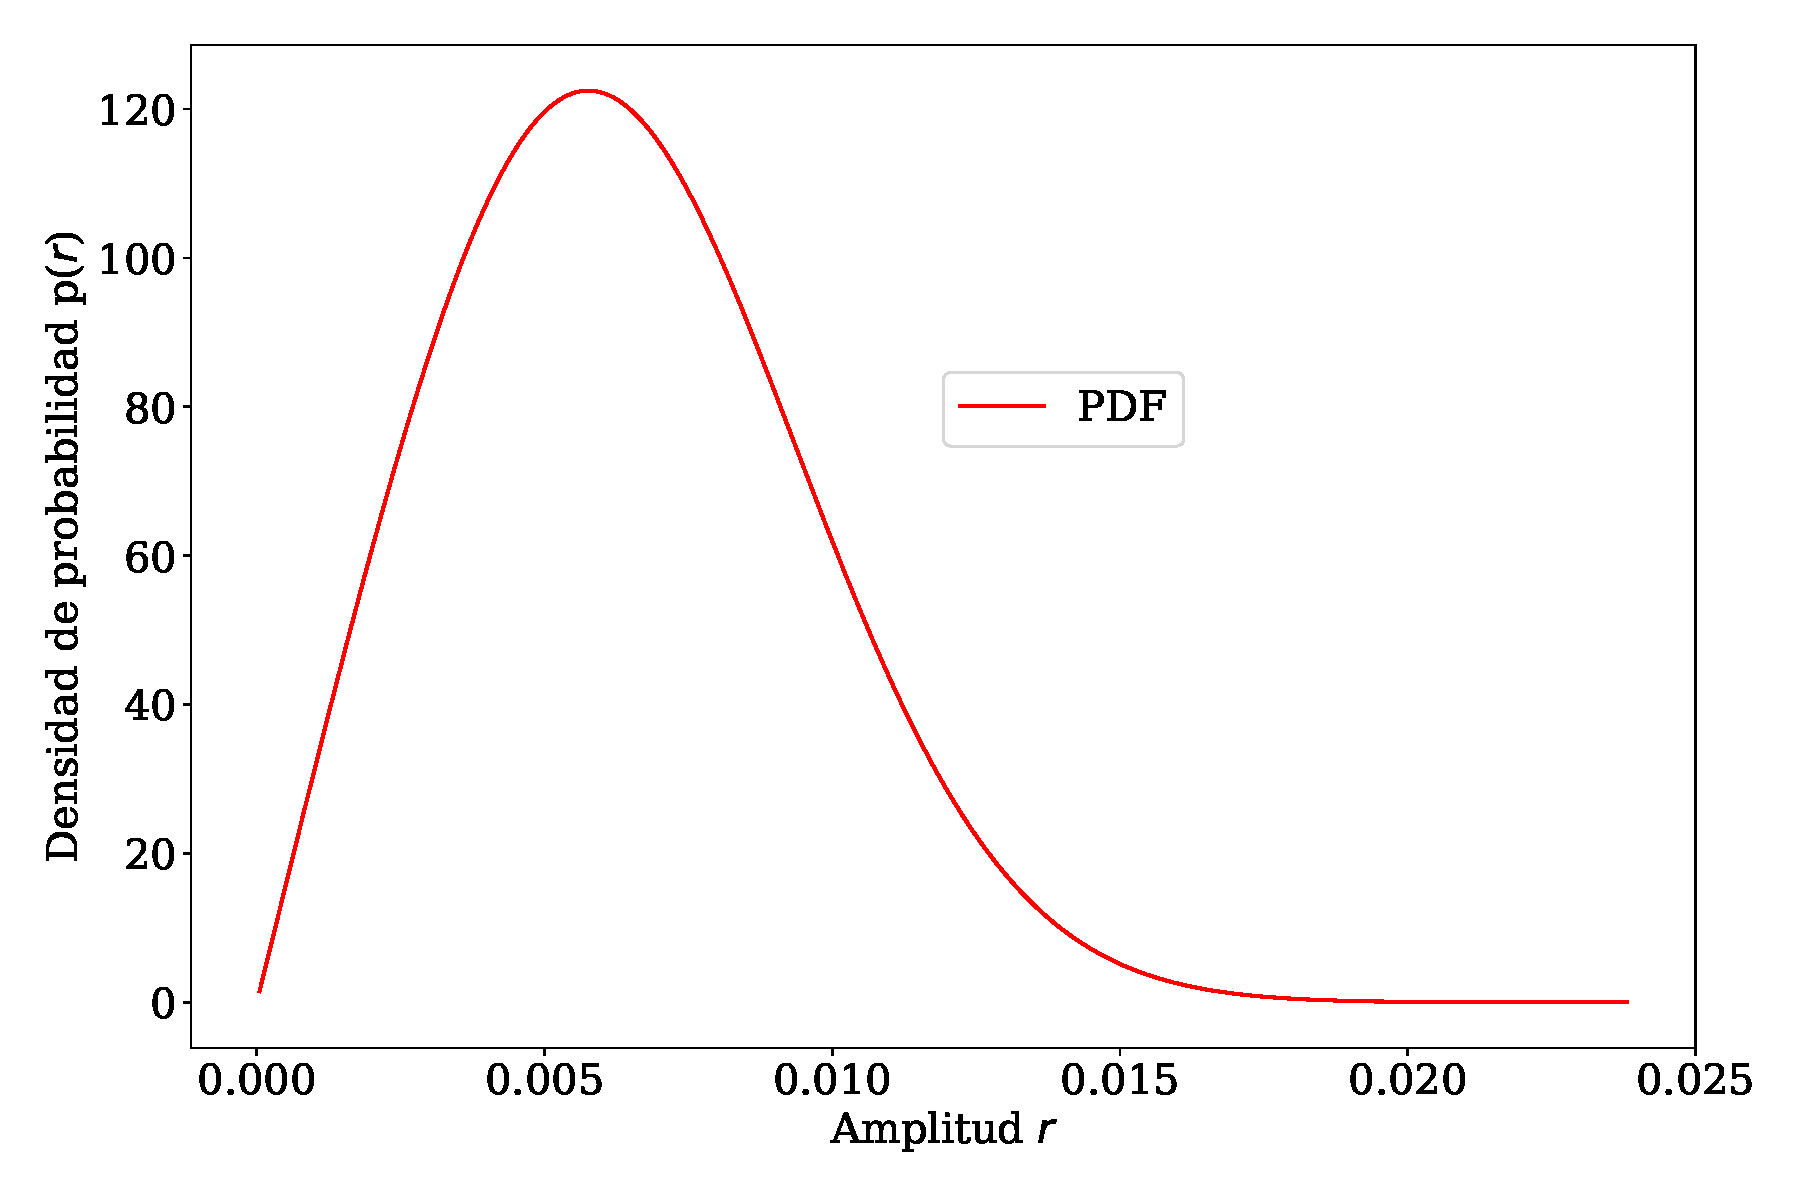
\includegraphics[width=0.75\textwidth]{bessel_prob_v2.pdf}
        \end{center}
        \caption{El gráfico de la función $p(r)$ y el límite de confianza para $s=0.005$ y $\sigma=0.038$ }
    \end{small}
\end{figure}

Esta figura nos dice por ejemplo que la probabilidad que el dípolo físico se encuentre entre $0$ y $0.015$ es del $85\%$.

\subsection{Haciendo la cuenta de los márgenes de confianza de la amplitud}

(???)Calculemos los márgenes de confianza para el ejemplo anterior de $s=0.005$ y $\sigma=0.038$. En este trabajo los márgenes que se obtuvieron nos dicen que el nivel de confianza en ese intervalo del $68.27\%$, dado que si N fuera muy grande, la pdf tiende a una gaussiana y el nivel de confianza sería a una sigma.


Los pasos que sigo son los siguientes: 

\begin{enumerate}
    \item 
    Dado que la pdf tiene una función de bessel modificada de primer orden que diverge en el 0, se toma una aproximación a la función con los primeros 8 términos de la sucesión. (agregar el anexo). Por ende la pdf no está normalizada. 
    
    Para normalizarla calculo la probabilidad asociada a $r_{max}=r +  10\sigma$. Dado que está tan alejada del valor de amplitud obtenida, el CL$\simeq 1$, por lo que uso este valor para normalizar  la Ec. \ref{ec:pdf} en el código.
    \item Una vez que tengo la función normalizada, finalmente hago la integral de la ecuación \ref{ec:integral} $CL(0,s,s)$ hasta un valor inicial de $s$ y el valor de la función $p(s)=p_1$.
    \begin{figure}[H]
        \begin{small}
            \begin{center}
                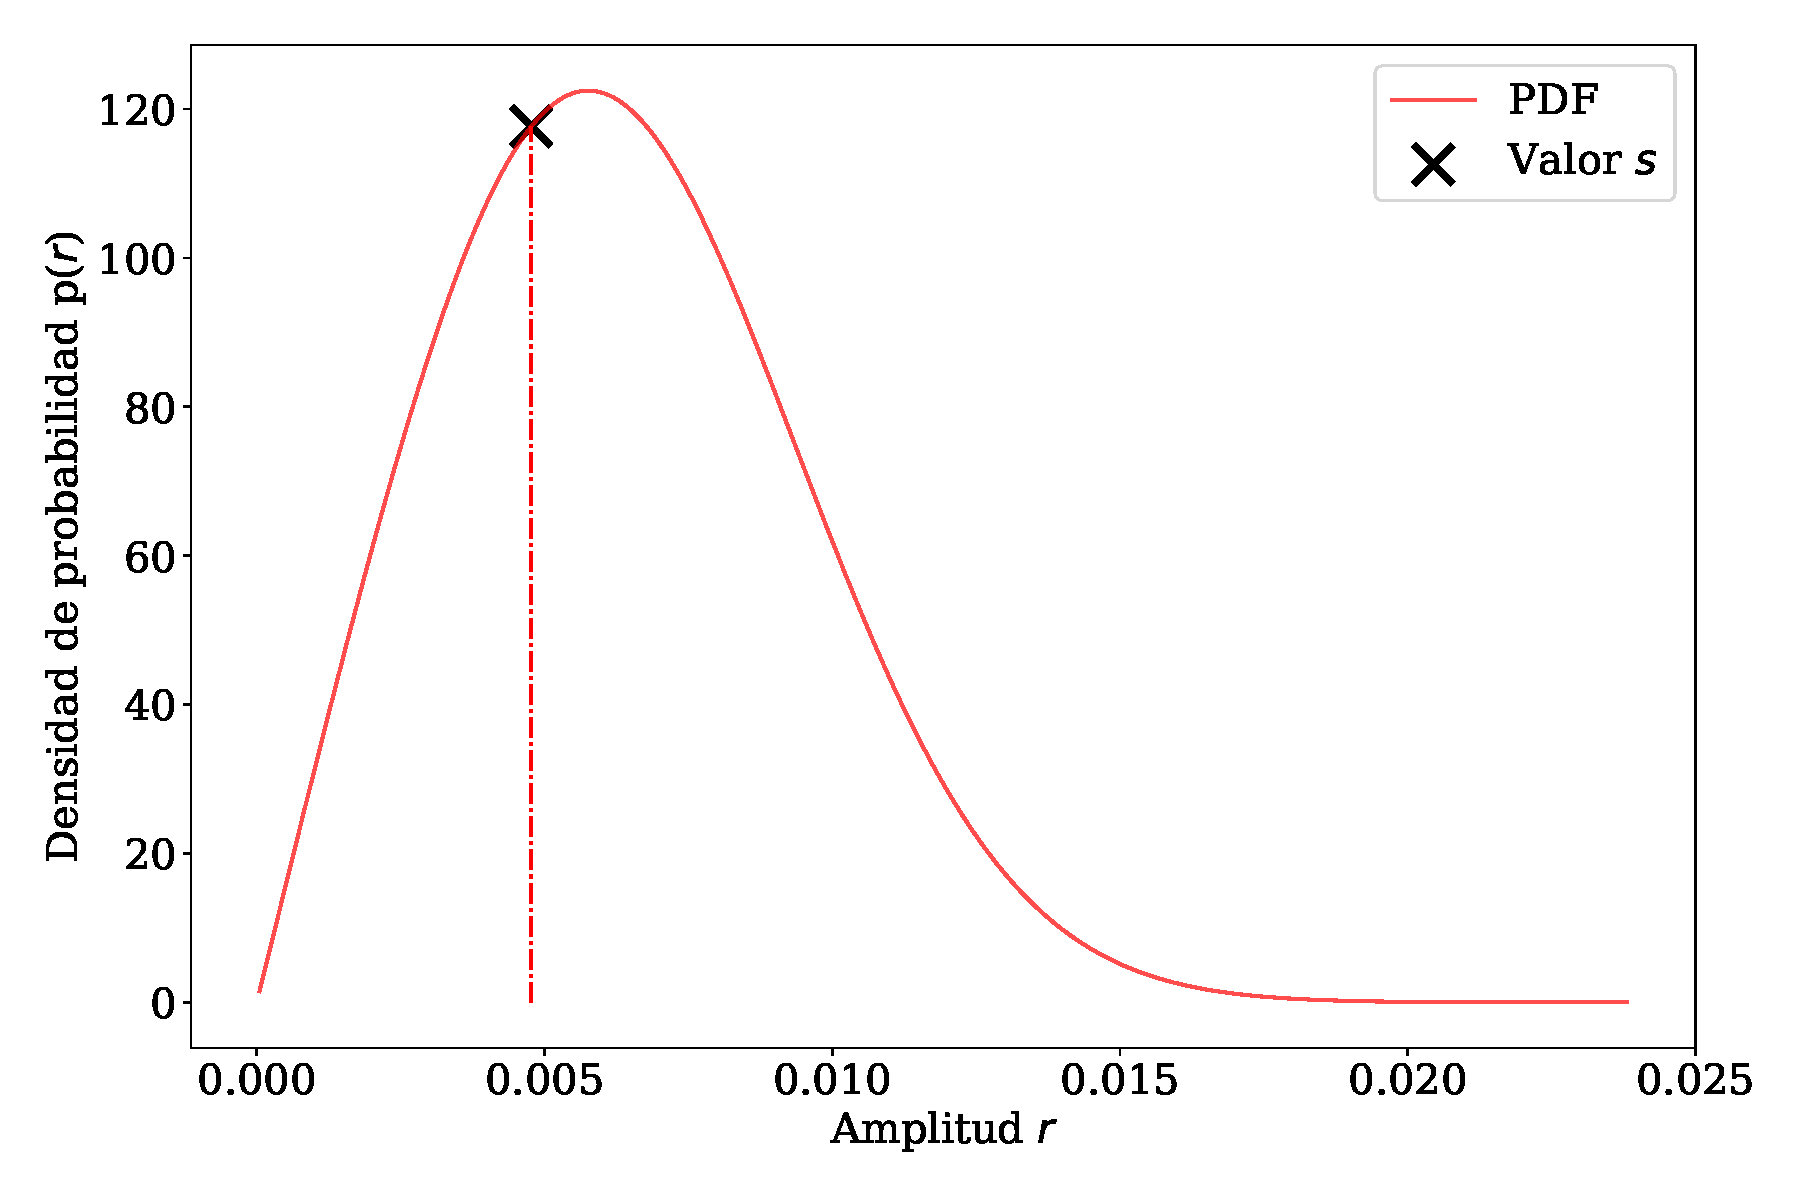
\includegraphics[width=0.75\textwidth]{bessel_prob_value_s_v2.pdf}
            \end{center}
            \caption{}
        \end{small}
    \end{figure}
    \item Si $CL(0,s,s)< 0.683$:
    \begin{enumerate}
        \item Teniendo en cuenta el valor inicial de $p_1$, se actualiza el valor  $p_2 \leftarrow p_1 - 0.01 p_1$ \label{itm:1}.
        \item Se calcula la integral entre los dos puntos con valores igual a $p(r)_2$. 
        \item \label{itm:3} Si la integral es menor a $0.6827$, se repite el proceso desde el paso \ref{itm:1}. Caso contrario, si esta integral es mayor o igual a $0.6827$, se calculan los valores límites de $r$ mediante el valor $p_2$ en el siguiente paso. 

        \begin{figure}[H]
            \begin{small}
                \begin{center}
                    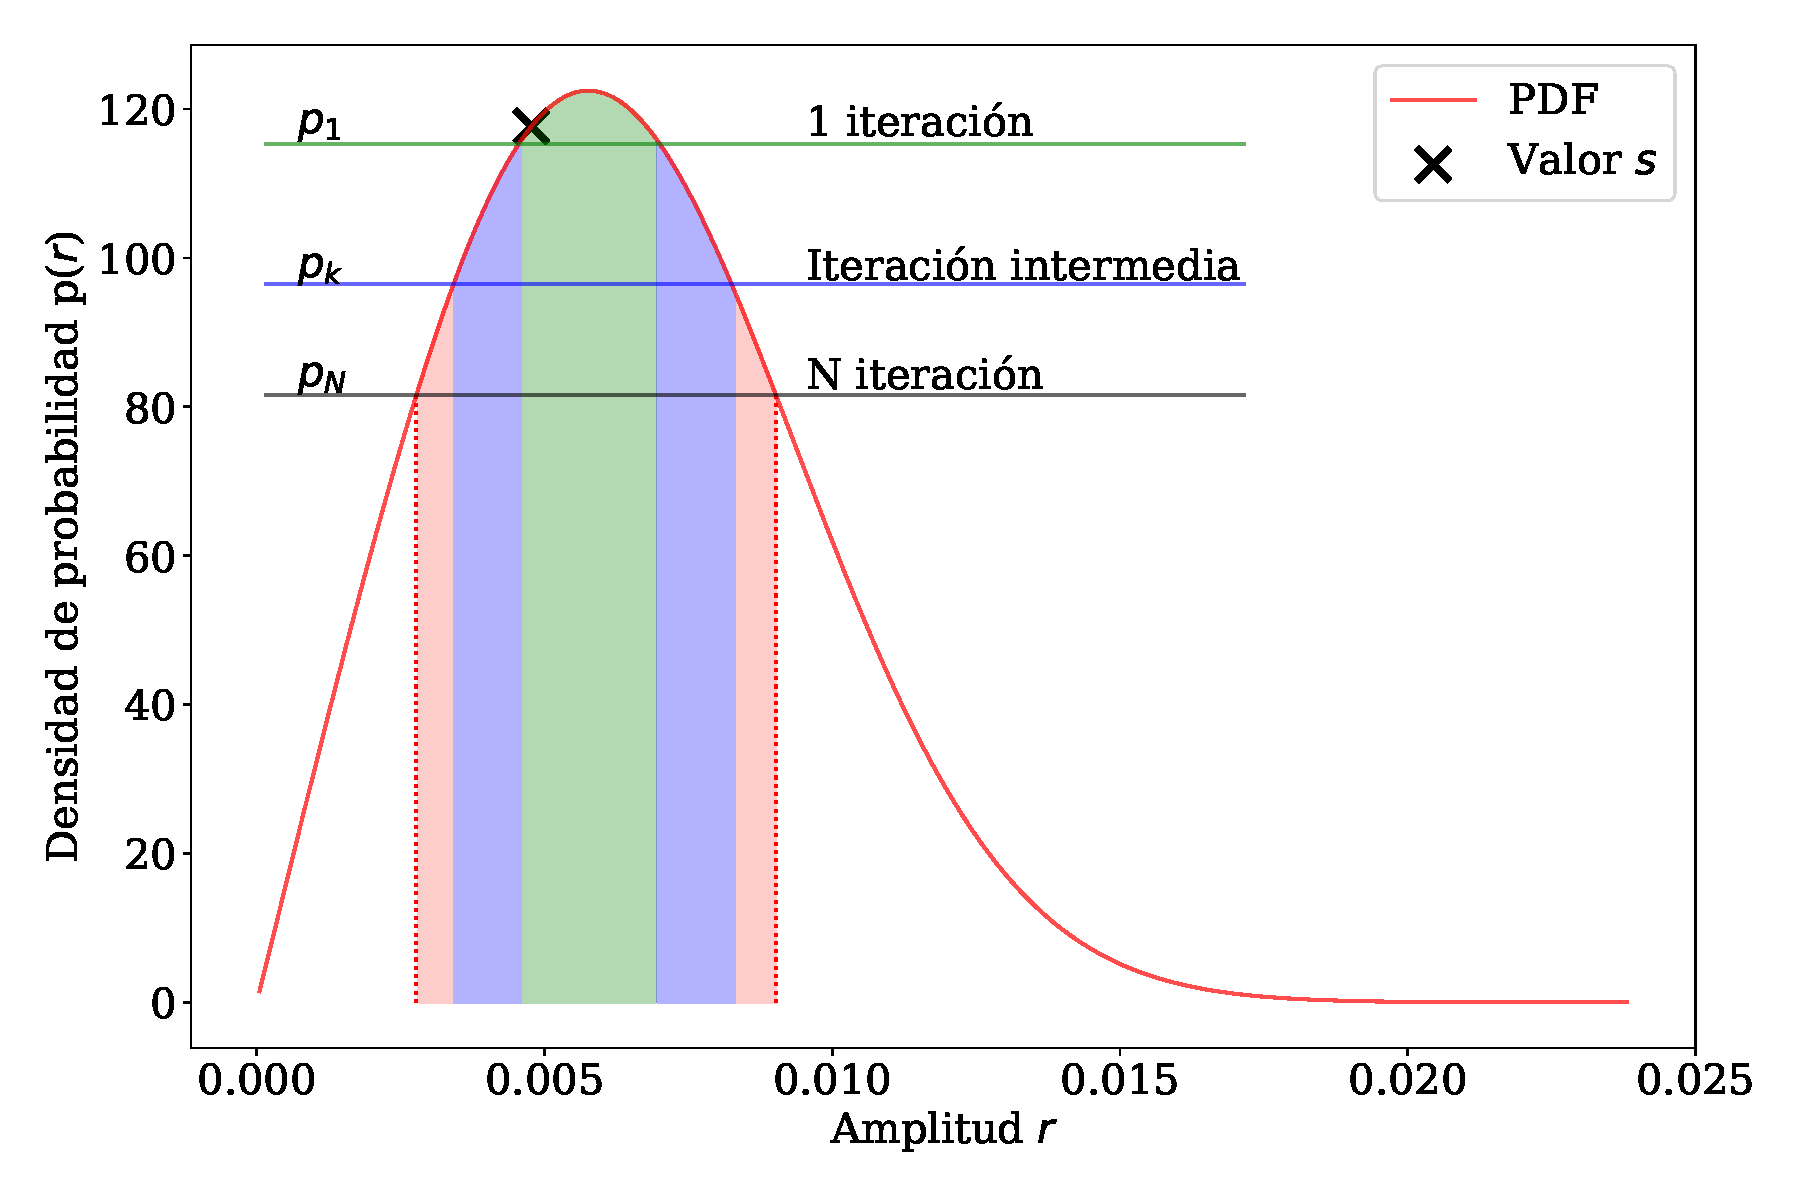
\includegraphics[width=0.75\textwidth]{bessel_prob_iterations_v2.pdf}
                \end{center}
                \caption{}
            \end{small}
        \end{figure}
    \end{enumerate}
    \item Si $CL(0,s,s)> 0.683$:
    \begin{enumerate}
        \item Se toma como límite inferior $r^-$el valor $s$ y se busca el límite superior $r^+$ de tal forma que $CL(s,s+\sigma^+,s) \simeq 0.683$. En este  trabajo no se encontró este caso pero se menciona por completitud ya  que está implementado en el código del trabajo \cite{Aab_2020}.
    \end{enumerate}
    \item Para calcular los límites de confianza superior $r^+$  y inferior $r^-$, teniendo en cuenta el valor final $p_N$ del paso \ref{itm:3}, se calculan los valores de $r_i$ donde se cumple que $p(r_i)=p_N$, los mismos son $r^+$  y  $r^-$. Finalmente los límites de confianza se calculan como:
    \begin{align*}
        \sigma^- = s-r^-\\
        \sigma^+ = s^+ -r
    \end{align*}
\end{enumerate}

\begin{figure}[H]
    \begin{small}
        \begin{center}
            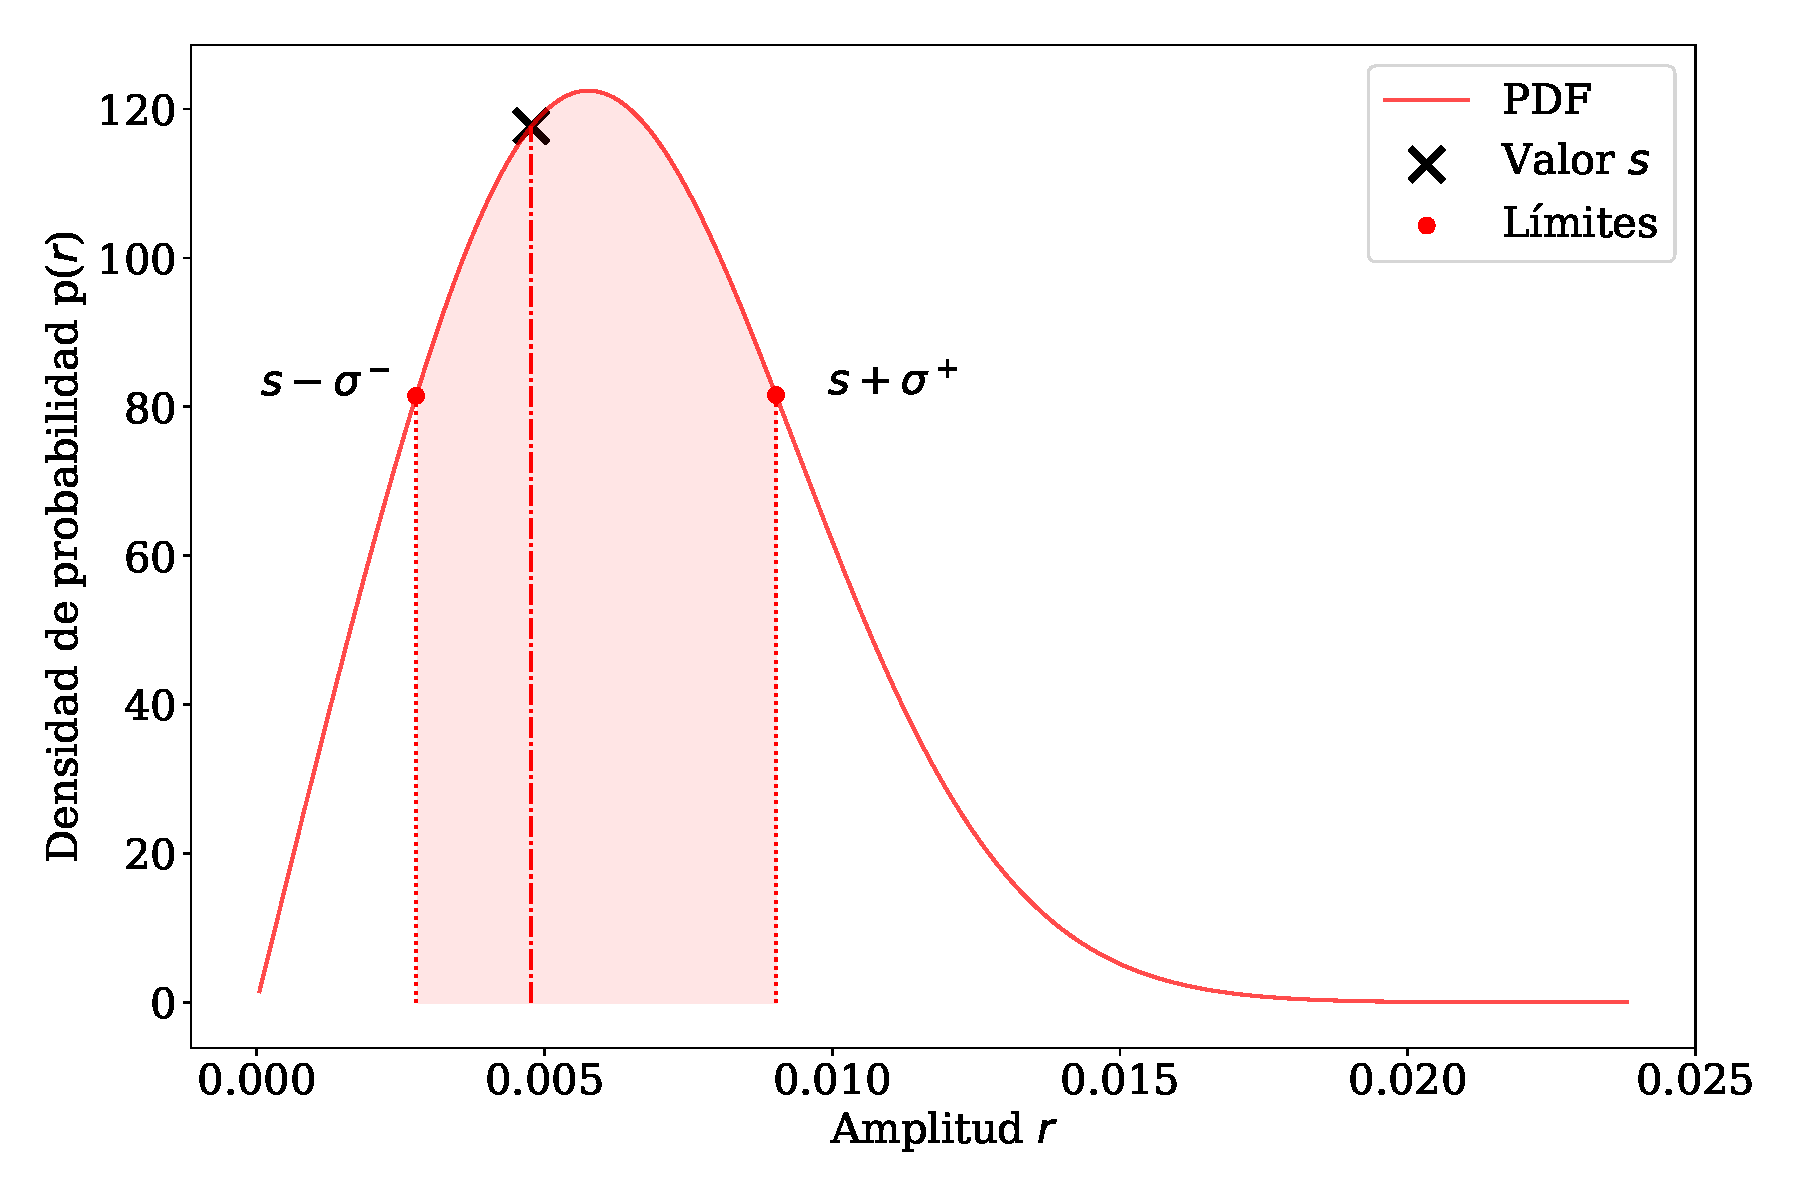
\includegraphics[width=0.75\textwidth]{bessel_prob_ej_v2.pdf}
        \end{center}
        \caption{}
    \end{small}
\end{figure}

\section{Distribución de probabilidad de la  fase del dipolo}

Si ahora se integra la ecuación \ref{eq:full_pdf} se obtiene la distribución de probabilidad de la fase $\psi$ de la Ec.\ref{eq:phase_pdf}.  

\begin{align}
    p(\psi) &=d\psi\,\frac{1}{2\pi}e^{-k} \Bigg[ 1 + (\pi k)^{\nicefrac{1}{2}} \cos\psi e^{(k\cos^2\psi)} \Big( 1 + L \erf(L k^{\nicefrac{1}{2}} \cos\psi \Big) \Bigg ] \\ \label{eq:phase_pdf}
    CL_{\psi}(\phi_1, \phi_2, s) &= \int_{\phi_1}^{\phi_2} d\psi \, p(\psi)
\end{align}  
donde $k =\nicefrac{s^2}{\sigma^2}$ y $\erf (x)$ es la función error, y
\begin{align*}
    L =
    \begin{cases} 
        +1 & \text{ Si } -\frac{\pi}{2} \geq x\leq \frac{\pi}{2} \\
        -1 & \text{ Caso contrario }  \\
     \end{cases}
\end{align*}

La distribución de probabilidad tiene la característica  de ser simétrica respecto a 0, por eso los límites de integración son $[-\pi, \pi]$.

Se definió que el nivel de confianza para la fase reportada en este trabajo sea del $95.45\%$d, ya que $k>>1$ la distribución de la fase se acerca a una distribución normal y este nivel de confianza es equivalente a $2\sigma$. Para calcular  $CL_\psi$ dada la simétrica  con respecto al 0, se siguen los siguientes  pasos:

\begin{enumerate}
    \item Se toma un valor inicial de $\sigma{\psi,0}=0.01*|\psi|$, donde  $\psi$ es valor de fase obtenida ya sea por el método Rayleigh o East-West. Se eligió este valor inicial por conveniencia.
    \item Se integra la Ec.\ref{eq:phase_pdf} en el rango $[-\sigma_{\psi,0}, \sigma_{\psi,0}]$ y se verifica si $CL_{\psi}(-\sigma_{\psi,0}, \sigma_{\psi,0},s) = 0.9545$. \label{paso1}
    \item Si ese es el caso, se reporta la fase como $\psi \pm \sigma_{\psi,0}$, caso contrario se vuelve al paso anterior con $\sigma_{\psi,1} \leftarrow \sigma_{\psi,0} + 0.01\sigma_{\psi,0}$. \label{paso2}
    \item Se entre los pasos \ref{paso1} y \ref{paso2}  hasta obtener el valor de $\sigma_{\psi,N}$ que cumpla $CL_{\psi}(-\sigma_{\psi,N}, \sigma_{\psi,N},s) = 0.9545$
\end{enumerate}

En la Fig.\ref{fig:phase_prob_ej} se muestra la distribución de probabilidad de la fase para $s=0.005$ y $\sigma = 0.0038$, también se incluye los límites de confianza obtenidos.

\begin{figure}[H]
    \begin{small}
        \begin{center}
            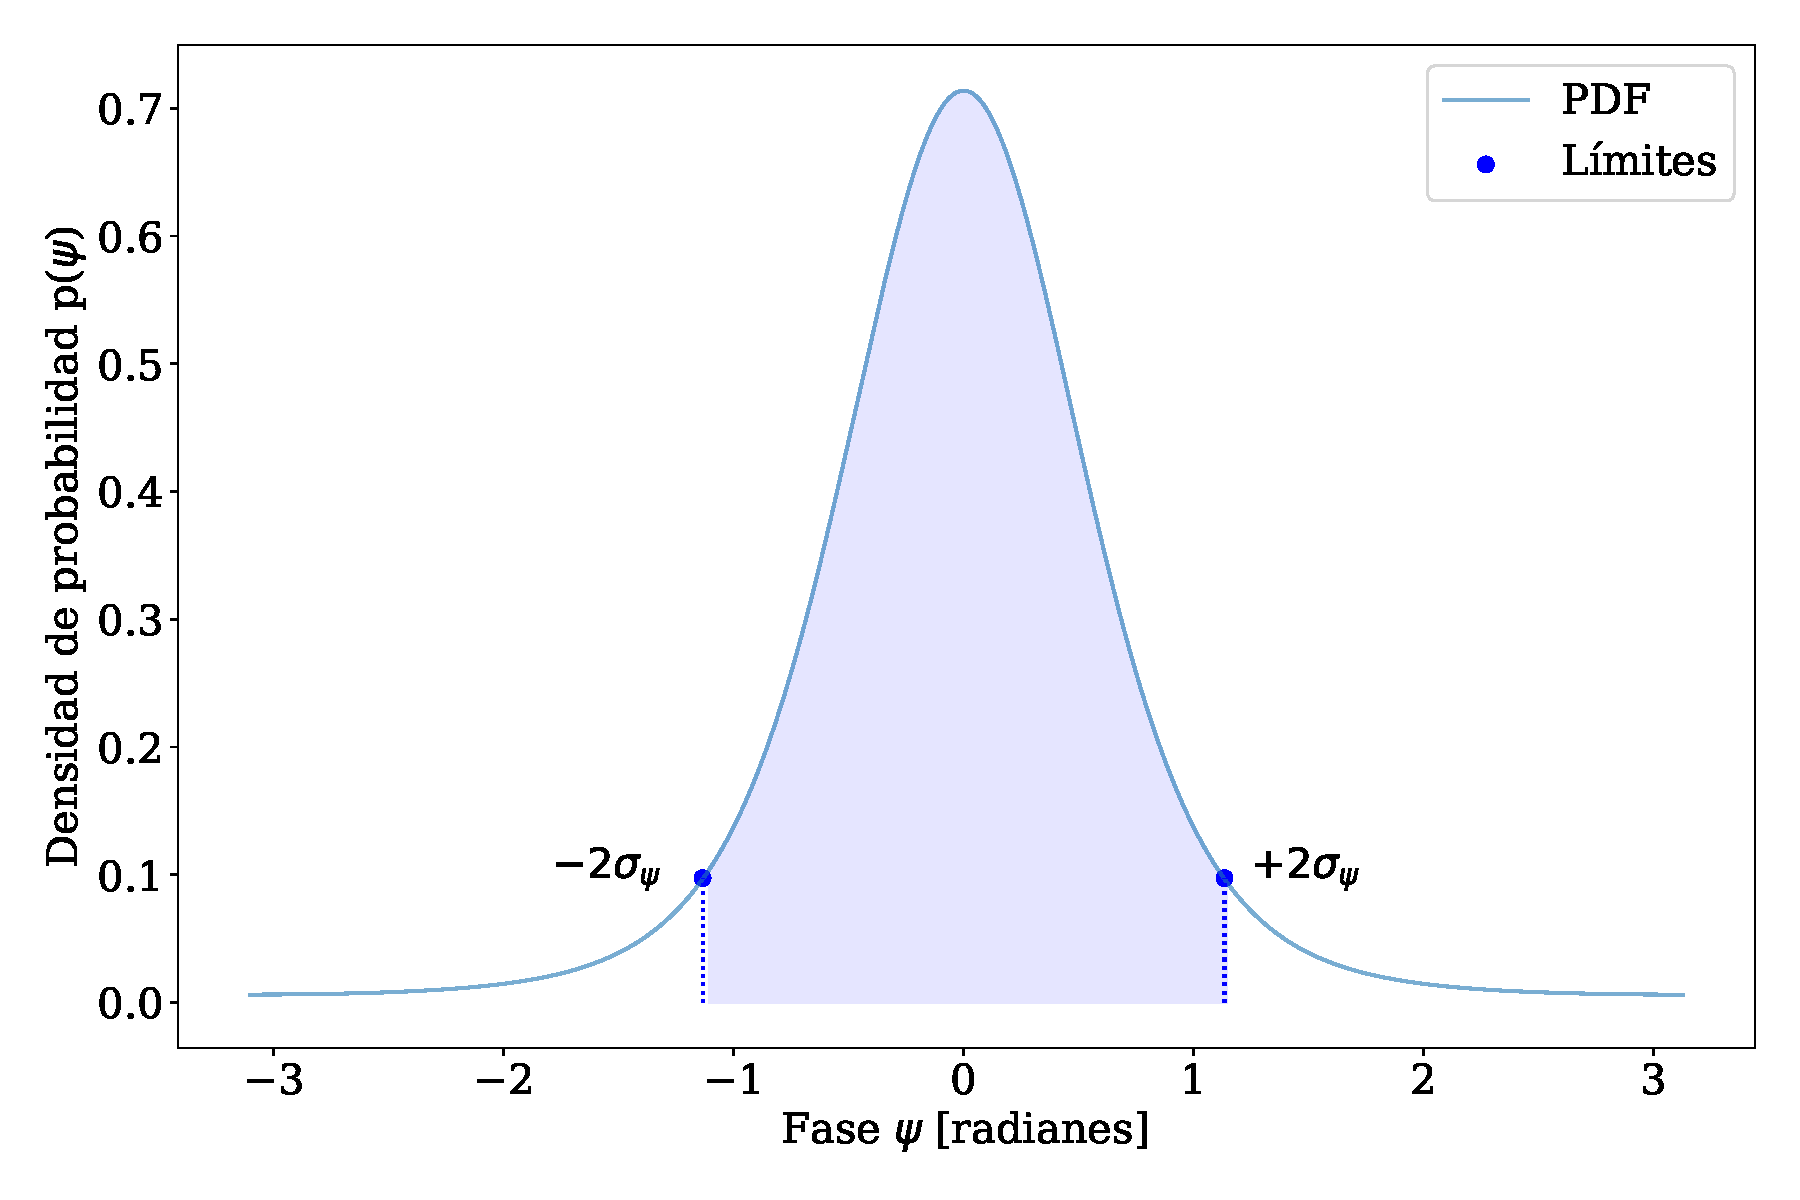
\includegraphics[width=0.75\textwidth]{phase_prob_ej.pdf}
        \end{center}
        \caption{La distribución de probabilidad de la fase para $s=0.005$ y $\sigma = 0.0038$ con los límites de confianza del $95.45\%$.}
        \label{fig:phase_prob_ej}
    \end{small}
\end{figure}